\documentclass[10pt]{beamer}

\newtheorem{conjecture}{Conjecture}
\newtheorem{exercise}{Exercise}

\setbeamertemplate{footline}[page number]

\title{Division polynomials of elliptic curves}

\author{David Kurniadi Angdinata (joint with Junyan Xu)}

\institute{London School of Geometry and Number Theory}

\date{Friday, 17 January 2025}

\begin{document}

\frame{\titlepage}

\begin{frame}[t]{Elliptic curves}

An elliptic curve over a field $ F $ is a smooth projective curve $ E $ of genus one, equipped with a fixed point $ \mathcal{O} $ defined over $ F $.

\begin{center}
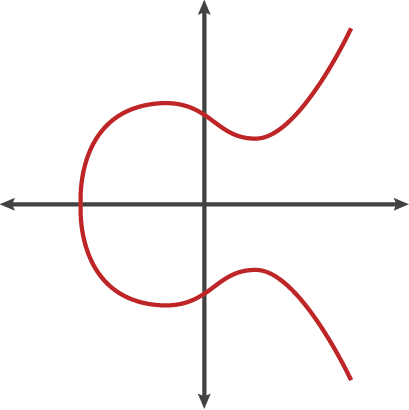
\includegraphics[width=0.5\textwidth]{ellipticcurves.png}
\end{center}

They are one of the simplest non-trivial objects in arithmetic geometry.

\end{frame}

\begin{frame}[t]{Weierstrass equations}

In \texttt{mathlib}, an \textbf{elliptic curve} $ E $ over an integral domain $ R $ is a tuple $ (a_1, a_2, a_3, a_4, a_6) \in R^5 $, with an extra condition that $ \Delta \in R^\times $, where
\begin{align*}
b_2 & := a_1^2 + 4a_2, \\
b_4 & := 2a_4 + a_1a_3, \\
b_6 & := a_3^2 + 4a_6, \\
b_8 & := a_1^2a_6 + 4a_2a_6 - a_1a_3a_4 + a_2a_3^2 - a_4^2, \\
\Delta & := -b_2^2b_8 - 8b_4^3 - 27b_6^2 + 9b_2b_4b_6.
\end{align*}

\pause

A \textbf{point} on $ E $ is either $ \mathcal{O} $ or an \textbf{affine point} $ (x, y)_a \in R^2 $ such that
$$ y^2 + a_1xy + a_3y = x^3 + a_2x^2 + a_4x^3 + a_6, $$
so the points on $ E $ vanish on the polynomial $ \mathcal{E} \in R[X, Y] $ given by
$$ \mathcal{E} := Y^2 + a_1XY + a_3Y - (X^3 + a_2X^2 + a_4X + a_6). $$

\end{frame}

\begin{frame}[t]{Group law}

The points on $ E $ can be endowed with a geometric addition law.

\begin{center}
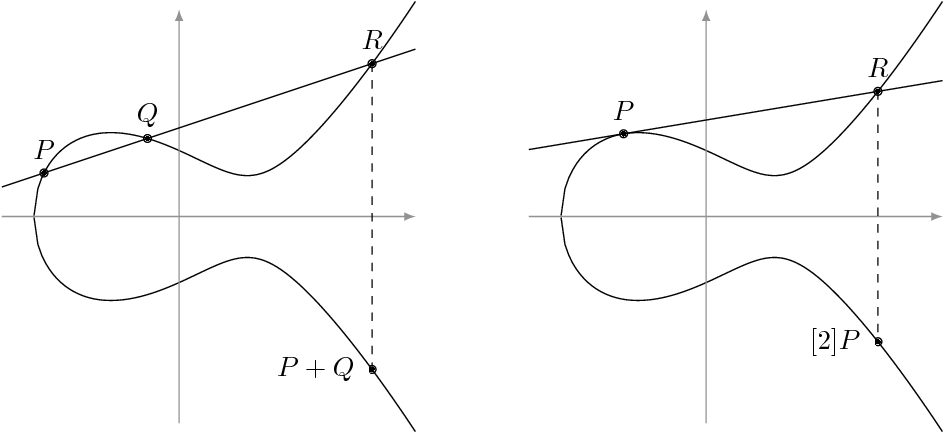
\includegraphics[width=\textwidth]{grouplaw.png}
\end{center}

\pause

In 2023, we formalised a novel algebraic proof of the group law on $ E $.

\pause

\vspace{0.5cm} Is there an explicit formula for $ [n]P $ in terms of $ P $?

\end{frame}

\begin{frame}[t]{An impossible exercise}

\emph{The Arithmetic of Elliptic Curves} by Silverman gives an answer.

\begin{exercise}[3.7(d)]
Let $ n \in \mathbb{Z} $. Prove that for any point $ (x, y)_a $ on $ E $,
$$ [n](x, y)_a = \left(\dfrac{\phi_n(x, y)}{\psi_n(x, y)^2}, \dfrac{\omega_n(x, y)}{\psi_n(x, y)^3}\right)_a. $$
\end{exercise}

Silverman gives inductive definitions for $ \phi_n, \omega_n, \psi_n \in F[X, Y] $.

\pause

\vspace{0.5cm} This formula leads to a proof that
$$ T_pE_{\overline{F}} \cong \begin{cases} \mathbb{Z}_p^2 & \mathrm{char}(F) \ne p \\ 0 \ \text{or} \ \mathbb{Z}_p & \mathrm{char}(F) = p \end{cases}. $$
These polynomials also feature in Schoof's algorithm.

\end{frame}

\begin{frame}[t]{Multiplication by $ 2 $}

If $ (x, y)_a $ is a generic affine point on $ E $, then
$$ [2](x, y)_a = \left(\dfrac{\phi_2(x, y)}{\psi_2(x, y)^2}, \dfrac{\omega_2(x, y)}{\psi_2(x, y)^3}\right)_a, $$
where $ \phi_2, \omega_2, \psi_2 \in F[X, Y] $ are given by
\begin{align*}
\psi_2 & := 2Y + a_1X + a_3, \\
\phi_2 & := X\psi_2^2 - \bigcirc, \\
\omega_2 & := \dfrac{1}{2}(\triangle - (a_1\phi_2 + a_3)\psi_2^3),
\end{align*}
for some $ \bigcirc, \triangle \in F[X] $. \pause If $ (x, y)_a $ is a $ 2 $-torsion affine point on $ E $, then
$$ (x, y)_a = -(x, y)_a = (x, -y - a_1x - a_3)_a, $$
so $ \psi_2(x, y) = 2y + a_1x + a_3 = 0 $.

\end{frame}

\begin{frame}[t]{Projective coordinates}

Let $ (x, y)_a $ be an affine point on $ E $. In \textbf{projective} coordinates,
$$ [2](x, y)_a = (\phi_2(x, y)\psi_2(x, y) : \omega_2(x, y) : \psi_2(x, y)^3)_p. $$
In \texttt{mathlib}, a \textbf{projective point} on $ E $ is a class of $ (x, y, z) \in F^3 $ such that
$$ y^2z + a_1xyz + a_3yz^2 = x^3 + a_2x^2z + a_4xz^2 + a_6z^3. $$
The point at infinity on $ E $ is $ (0 : 1 : 0)_p $.

\pause

\vspace{0.5cm} More naturally, in \textbf{Jacobian} coordinates with weights $ (2 : 3 : 1) $,
$$ [2](x, y)_a = (\phi_2(x, y) : \omega_2(x, y) : \psi_2(x, y))_j. $$
In \texttt{mathlib}, a \textbf{Jacobian point} on $ E $ is a class of $ (x, y, z) \in F^3 $ such that
$$ y^2 + a_1xyz + a_3yz^3 = x^3 + a_2x^2z^2 + a_4xz^4 + a_6z^6. $$
The point at infinity on $ E $ is $ (1 : 1 : 0)_j $.

\end{frame}

\begin{frame}[t]{Multiplication by $ n $}

\begin{exercise}[3.7(d), corrected]
Let $ n \in \mathbb{Z} $. Prove that for any point $ (x, y)_a $ on $ E $,
$$ [n](x, y)_a = (\phi_n(x, y) : \omega_n(x, y) : \psi_n(x, y))_j. $$
\end{exercise}

\pause

If $ (x : y : z)_j $ is a point on $ E $, then $ x = y = 1 $ whenever $ z = 0 $, so
$$ \ker[n] = \{\mathcal{O}\} \cup \{(x, y)_a \mid \psi_n(x, y) = 0\}. $$

\pause

\begin{conjecture}
No one has done Exercise 3.7(d) purely inductively.
\end{conjecture}

\pause

\vspace{0.5cm} Xu gave a complete answer to this exercise and formalised it in Lean.

\vspace{0.5cm} I will define $ \phi_n $, $ \omega_n $, $ \psi_n $, and their auxiliary polynomials.

\end{frame}

\begin{frame}[t]{The polynomials $ \psi_n $}

The $ n $-th \textbf{division polynomial} $ \psi_n \in R[X, Y] $ is given by
\begin{align*}
\psi_0 & := 0, \\
\psi_1 & := 1, \\
\psi_2 & := 2Y + a_1X + a_3, \\
\psi_3 & := \bigcirc \\
& \qquad \text{where} \ \bigcirc := 3X^4 + b_2X^3 + 3b_4X^2 + 3b_6X + b_8, \\
\psi_4 & := \psi_2\triangle \\
& \qquad \text{where} \ \triangle := {\scriptscriptstyle 2X^6 + b_2X^5 + 5b_4X^4 + 10b_6X^3 + 10b_8X^2 + (b_2b_8 - b_4b_6)X + (b_4b_8 - b_6^2)}, \\
\psi_{2n + 1} & := \psi_{n + 2}\psi_n^3 - \psi_{n - 1}\psi_{n + 1}^3, \\
\psi_{2n} & := \dfrac{\psi_{n - 1}^2\psi_n\psi_{n + 2} - \psi_{n - 2}\psi_n\psi_{n + 1}^2}{\psi_2}, \\
\psi_{-n} & := -\psi_n.
\end{align*}
In \texttt{mathlib}, $ \psi_n $ is defined in terms of $ \Psi_n \in R[X] $.

\end{frame}

\begin{frame}[t]{The polynomials $ \Psi_n $}

The polynomial $ \Psi_n \in R[X] $ is given by
\begin{align*}
\Psi_0 & := 0, \\
\Psi_1 & := 1, \\
\Psi_2 & := 1, \\
\Psi_3 & := \bigcirc, \\
\Psi_4 & := \triangle, \\
\Psi_{2n + 1} & := \begin{cases} \Psi_{n + 2}\Psi_n^3 - \square^2\Psi_{n - 1}\Psi_{n + 1}^3 & \text{if} \ n \ \text{is odd} \\ \square^2\Psi_{n + 2}\Psi_n^3 - \Psi_{n - 1}\Psi_{n + 1}^3 & \text{if} \ n \ \text{is even} \end{cases} \\
& \qquad \text{where} \ \square := 4X^3 + b_2X^2 + 2b_4X + b_6, \\
\Psi_{2n} & := \Psi_{n - 1}^2\Psi_n\Psi_{n + 2} - \Psi_{n - 2}\Psi_n\Psi_{n + 1}^2, \\
\Psi_{-n} & := -\Psi_n.
\end{align*}
Then $ \psi_n = \Psi_n $ when $ n $ is odd and $ \psi_n = \psi_2\Psi_n $ when $ n $ is even.

\end{frame}

\begin{frame}[t]{The polynomials $ \phi_n $ and $ \Phi_n $}

In the coordinate ring of $ E $,
\begin{align*}
\psi_2^2
& = (2Y + a_1X + a_3)^2 \\
& = 4(Y^2 + a_1XY + a_3Y) + a_1^2X^2 + 2a_1a_3X + a_3^2 \\
& \equiv \underbrace{4X^3 + b_2X^2 + 2b_4X + b_6}_\square \mod \mathcal{E}.
\end{align*}
In particular, $ \psi_n^2 $ and $ \psi_{n + 1}\psi_{n - 1} $ are congruent to polynomials in $ R[X] $.

\pause

\vspace{0.5cm} The polynomial $ \phi_n \in R[X, Y] $ is given by
$$ \phi_n := X\psi_n^2 - \psi_{n + 1}\psi_{n - 1}, $$
so that $ \phi_n \equiv \Phi_n \mod \mathcal{E} $, where $ \Phi_n \in R[X] $ is given by
$$ \Phi_n := \begin{cases} X\Psi_n^2 - \square\Psi_{n + 1}\Psi_{n - 1} & \text{if} \ n \ \text{is odd} \\ X\square\Psi_n^2 - \Psi_{n + 1}\Psi_{n - 1} & \text{if} \ n \ \text{is even} \end{cases}. $$

\end{frame}

\begin{frame}[t]{The polynomials $ \omega_n $}

The polynomial $ \omega_n \in R[X, Y] $ is given by
$$ \omega_n := \dfrac{1}{2}\left(\dfrac{\psi_{2n}}{\psi_n} - a_1\phi_n\psi_n - a_3\psi_n^3\right). $$

\pause

\begin{lemma}[Xu]
Let $ n \in \mathbb{Z} $. Then $ \psi_{2n} / \psi_n - a_1\phi_n\psi_n - a_3\psi_n^3 $ is divisible by $ 2 $ in $ \mathbb{Z}[a_i, X, Y] $.
\end{lemma}

\pause

\begin{example}[$ a_1 = a_3 = 0 $]
\vspace{-0.5cm}
$$ \omega_2 = \dfrac{\Psi_4}{2} = \dfrac{\scriptstyle 2X^6 + 4a_2X^5 + 10a_4X^4 + 40a_6X^3 + 10b_8X^2 + (4a_2b_8 - 8a_4a_6)X + (2a_4b_8 - 16a_6^2)}{2}. $$
\end{example}

\pause

\vspace{0.5cm} Define $ \omega_n $ as the image of the quotient under $ \mathbb{Z}[a_i, X, Y] \to R[X, Y] $.

\pause

\vspace{0.5cm} When $ n = 4 $, this quotient has 15,049 terms.

\end{frame}

\begin{frame}[t]{Elliptic divisibility sequences}

Integrality relies on the fact that $ \psi_n $ is an \textbf{elliptic divisibility sequence}.

\begin{exercise}[3.7(g)]
For all $ n, m, r \in \mathbb{Z} $, prove that $ \psi_n \mid \psi_{nm} $ and
$$ \psi_{n + m}\psi_{n - m}\psi_r^2 = \psi_{n + r}\psi_{n - r}\psi_m^2 - \psi_{m + r}\psi_{m - r}\psi_n^2. $$
\end{exercise}

Note that this generalises the recursive definitions of $ \psi_{2n + 1} $ and $ \psi_{2n} $.

\pause

\vspace{0.5cm} Surprisingly, this needs the stronger result that $ \psi_n $ is an \textbf{elliptic net}.

\begin{theorem}[Xu]
Let $ n, m, r, s \in \mathbb{Z} $. Then
$$ \psi_{n + m}\psi_{n - m}\psi_{r + s}\psi_{r - s} = \psi_{n + r}\psi_{n - r}\psi_{m + s}\psi_{m - s} - \psi_{m + r}\psi_{m - r}\psi_{n + s}\psi_{n - s}. $$
\end{theorem}

\pause

Xu gave an elegant proof of this on Math Stack Exchange.

\end{frame}

\begin{frame}[t]{The Somos-4 invariant}

\only<1-6>{As an elliptic sequence, $ \psi_n $ satisfies the \textbf{Somos-4 recurrence}
$$ \psi_{n + 2}\psi_{n - 2} = \psi_2^2\psi_{n + 1}\psi_{n - 1} - \psi_3\psi_n^2. $$}

\only<2-6>{An easy induction gives an invariant
$$ \mathcal{I}(n) := \dfrac{\psi_{n - 1}^2\psi_{n + 2} + \psi_{n - 2}\psi_{n + 1}^2 + \psi_2^2\psi_n^3}{\psi_{n + 1}\psi_n\psi_{n - 1}}. $$}

\only<3-6>{When $ n = 2 $, \visible<4-6>{an explicit computation gives}
$$ \mathcal{I}(2) = \dfrac{\psi_4 + \psi_2^5}{\psi_3\psi_2} \visible<4-6>{\equiv a_1\psi_2 \mod 2.} $$}

\only<5-6>{Being an invariant means that $ \mathcal{I}(n) = \mathcal{I}(2) $, so}
\only<5>{$$ \dfrac{\psi_{n - 1}^2\psi_{n + 2} + \psi_{n - 2}\psi_{n + 1}^2 + \psi_2^2\psi_n^3}{\psi_{n + 1}\psi_n\psi_{n - 1}} \equiv a_1\psi_2 \mod 2. $$}
\only<6>{$$ \dfrac{\psi_{n - 1}^2\psi_{n + 2} + \psi_{n - 2}\psi_{n + 1}^2 + \psi_2^2\psi_n^3}{\psi_2} \equiv a_1\psi_{n + 1}\psi_n\psi_{n - 1} \mod 2. $$}

\end{frame}

\begin{frame}[t]{Integrality of $ \omega_n $}

In particular,
\begin{align*}
\dfrac{\psi_{2n}}{\psi_n}
& = \dfrac{\psi_{n - 1}^2\psi_{n + 2} - \psi_{n - 2}\psi_{n + 1}^2}{\psi_2} & \text{by definition of} \ \psi_{2n} \\
& \equiv \psi_2\psi_n^3 + a_1\psi_{n + 1}\psi_n\psi_{n - 1} \mod 2 & \text{by} \ \mathcal{I}(n) = \mathcal{I}(2) \\
& = 2Y\psi_n^3 + a_1(\underbrace{X\psi_n^2 + \psi_{n + 1}\psi_{n - 1}}_{\phi_n})\psi_n + a_3\psi_n^3 & \text{by definition of} \ \psi_2.
\end{align*}
Thus $ \psi_{2n} / \psi_n - a_1\phi_n\psi_n - a_3\psi_n^3 \equiv 0 \mod 2 $. \pause In Lean,
\begin{align*}
\omega_n
& := \dfrac{\psi_{n + 1}\psi_n\psi_{n - 1}}{\psi_2\psi_3}(4\mathcal{E}(2\mathcal{E} + \square) + \psi_3(a_1\psi_2 - \tfrac{\partial\mathcal{E}}{\partial X})) \\
& \qquad - \dfrac{\psi_{n - 2}\psi_{n + 1}^2}{\psi_2} + (Y - \psi_2)\psi_n^3,
\end{align*}
which is well-defined, since $ \psi_n $ is a divisibility sequence.

\end{frame}

\begin{frame}[t]{Other formalised results}

The polynomial $ \Psi_n^{(2)} \in R[X] $ is given by
$$ \Psi_n^{(2)} := \begin{cases} \Psi_n^2 & \text{if} \ n \ \text{is odd} \\ \square\Psi_n^2 & \text{if} \ n \ \text{is even} \end{cases}, $$
so that $ \Psi_2^{(2)} = \square $ and $ \Psi_n^{(2)} \equiv \psi_n^2 \mod \mathcal{E} $.

\pause

\vspace{0.5cm}

\begin{exercise}[3.7(b)]
Show that $ \Phi_n = X^{n^2} + \dots $ and $ \Psi_n^{(2)} = n^2X^{n^2 - 1} + \dots $.
\end{exercise}

This is an inductive computation of \texttt{natDegree} and \texttt{leadingCoeff}.

\pause

\vspace{0.5cm}

\begin{exercise}[3.7(c)]
Prove that $ \Phi_n $ and $ \Psi_n^{(2)} $ are relatively prime.
\end{exercise}

Surprisingly, this needs Exercise 3.7(d) and the assumption that $ \Delta \ne 0 $.

\end{frame}

\end{document}